\chapter{Data Collection and Management}
The first step in building any machine learning model is collecting, or acquiring, data to train and develop a model with. In order to collect user data there were also ethical considerations to take into account and ethics approval was required. This chapter will discuss the data collection process, and how the data was managed and stored for use in the project, and the ethical considerations and concerns that were a part of that data collection and storage development.

\section{Research Ethics Considerations and Approval}
When collecting data from participants, it is important to consider the ethical implications of that data collection. This is especially true when the data being collected is personal data, such as the data collected in this project. The data collected in this project was personal data, as it included information about the user's training sessions, including in many cases heart rate and GPS data, and their personal details such as their name and email address. As such, it was important to consider the ethical implications of collecting this data, and to ensure that the data was collected in a way that was respectful of the user's privacy and rights. Furthermore, all of the participants are active competitors, many of them competing against the researcher in the same events, so it was important to ensure that the data collected was not used in any way that could be seen as an unfair advantage. Some squads have strict policies surrounding the sharing of training data and scores, the same data privacy requirements were required to begin conversations with these squads and their members to collect data. 

When applying for ethics approval it was important to consider how user data could be protected both from unauthorised access, and, in the unlikely event of a data leak ensuring the exposure a user sees is minimal.

To ensure user data protection, much of the connection to an actual person is removed, the data is stored in a database with a unique identifier, and the user's email address is stored in a separate table. This means that if the database is accessed, the user's email address or other identifying information is not immediately available. The data is also stored in a secure database, with access restricted to only the researcher and the serverless functions that interact with the database. Any data is also encrypted at rest, and in transit, to ensure that it is secure. A table linking the unique identifiers generated for each user and identifiable user data was stored securely on the researchers personal machine making the de-pseudonymisation of the data more difficult. This key was kept in order to provide users feedback through the website, and to allow the researcher to delete any collected information if a user elected to leave the project early.

There was some GPS data available in some training sessions submitted as part of the project. It was determined that this data, if leaked, would not be a significant risk to the user, as the data was only collected during on the water training sessions where many rowers train and compete normally. As most rowers in a squad train together, if the raw data for multiple sessions were leaked it would be nearly impossible to pinpoint which sessions belonged to which athletes given the number of total athletes training at any one time. 

Most of the analytics approaches were tested using the researchers own training data. This ensured that the researcher did not get an unfair advantage when comparing to other athletes data, any further analytics done for individual users was done using serverless functions meaning the researcher never had direct access to the raw data. These policies and procedures were included in the ethics application, and were approved by the College Research Ethics Committee, and were shared with participants when in the recruitment stage. 

Following some difficulties with the new College Research Ethics Approval Management System (REAMS), an ethics approval application was submitted on November 2, 2023 and approval was granted on December 6, 2023.

\section{Data Collection}
When developing the data collection pipeline, some key considerations were made. Firstly, the user effort per activity logged was to be as minimal as possible. Rowers typically have a lot of data to log, and the more effort required to log each activity, the less likely they are to do so. In many cases they were already logging their training elsewhere as a part of their squad's training program, therefore making the process of logging their sessions for this project as seamless as possible became a priority. Next, for what little interaction was required, it was important that the platform be easy to use and intuitive. This was important as it reduced the workload to maintain the platform, by responding to user queries, and encouraged users to continue using the platform due to its easy of user.

Considering the minimum requirements for a successful data collection pipeline, a website was developed to manage data provider connections, and view training feedback. This website worked in conjunction with a series of serverless functions to automatically collect and analyse user sessions, and generate the feedback which was presented in the website.

\subsection{The Frontend}
The website was developed using Next.js, a React framework for building server-side rendered websites, it was developed using Typescript, which is a statically typed superset of JavaScript. This allowed for type checking and better code quality, and made it easier to develop and maintain the backend. It was designed to be simple and easy to use, with a focus on the user experience. This meant that the a mobile-first approach to design was needed, as many users would be accessing the website from their mobile devices, it also needed to be fast and lightweight meaning many of the data heavy components of the webapp are rendered with server-side components to reduce the client-side workload ensuring a smooth and consistent app experience. The webapp is also fairly basic, including only three screens once logged in.
\subsubsection{Login and Register}

\begin{figure}[htbp]
  \centering
  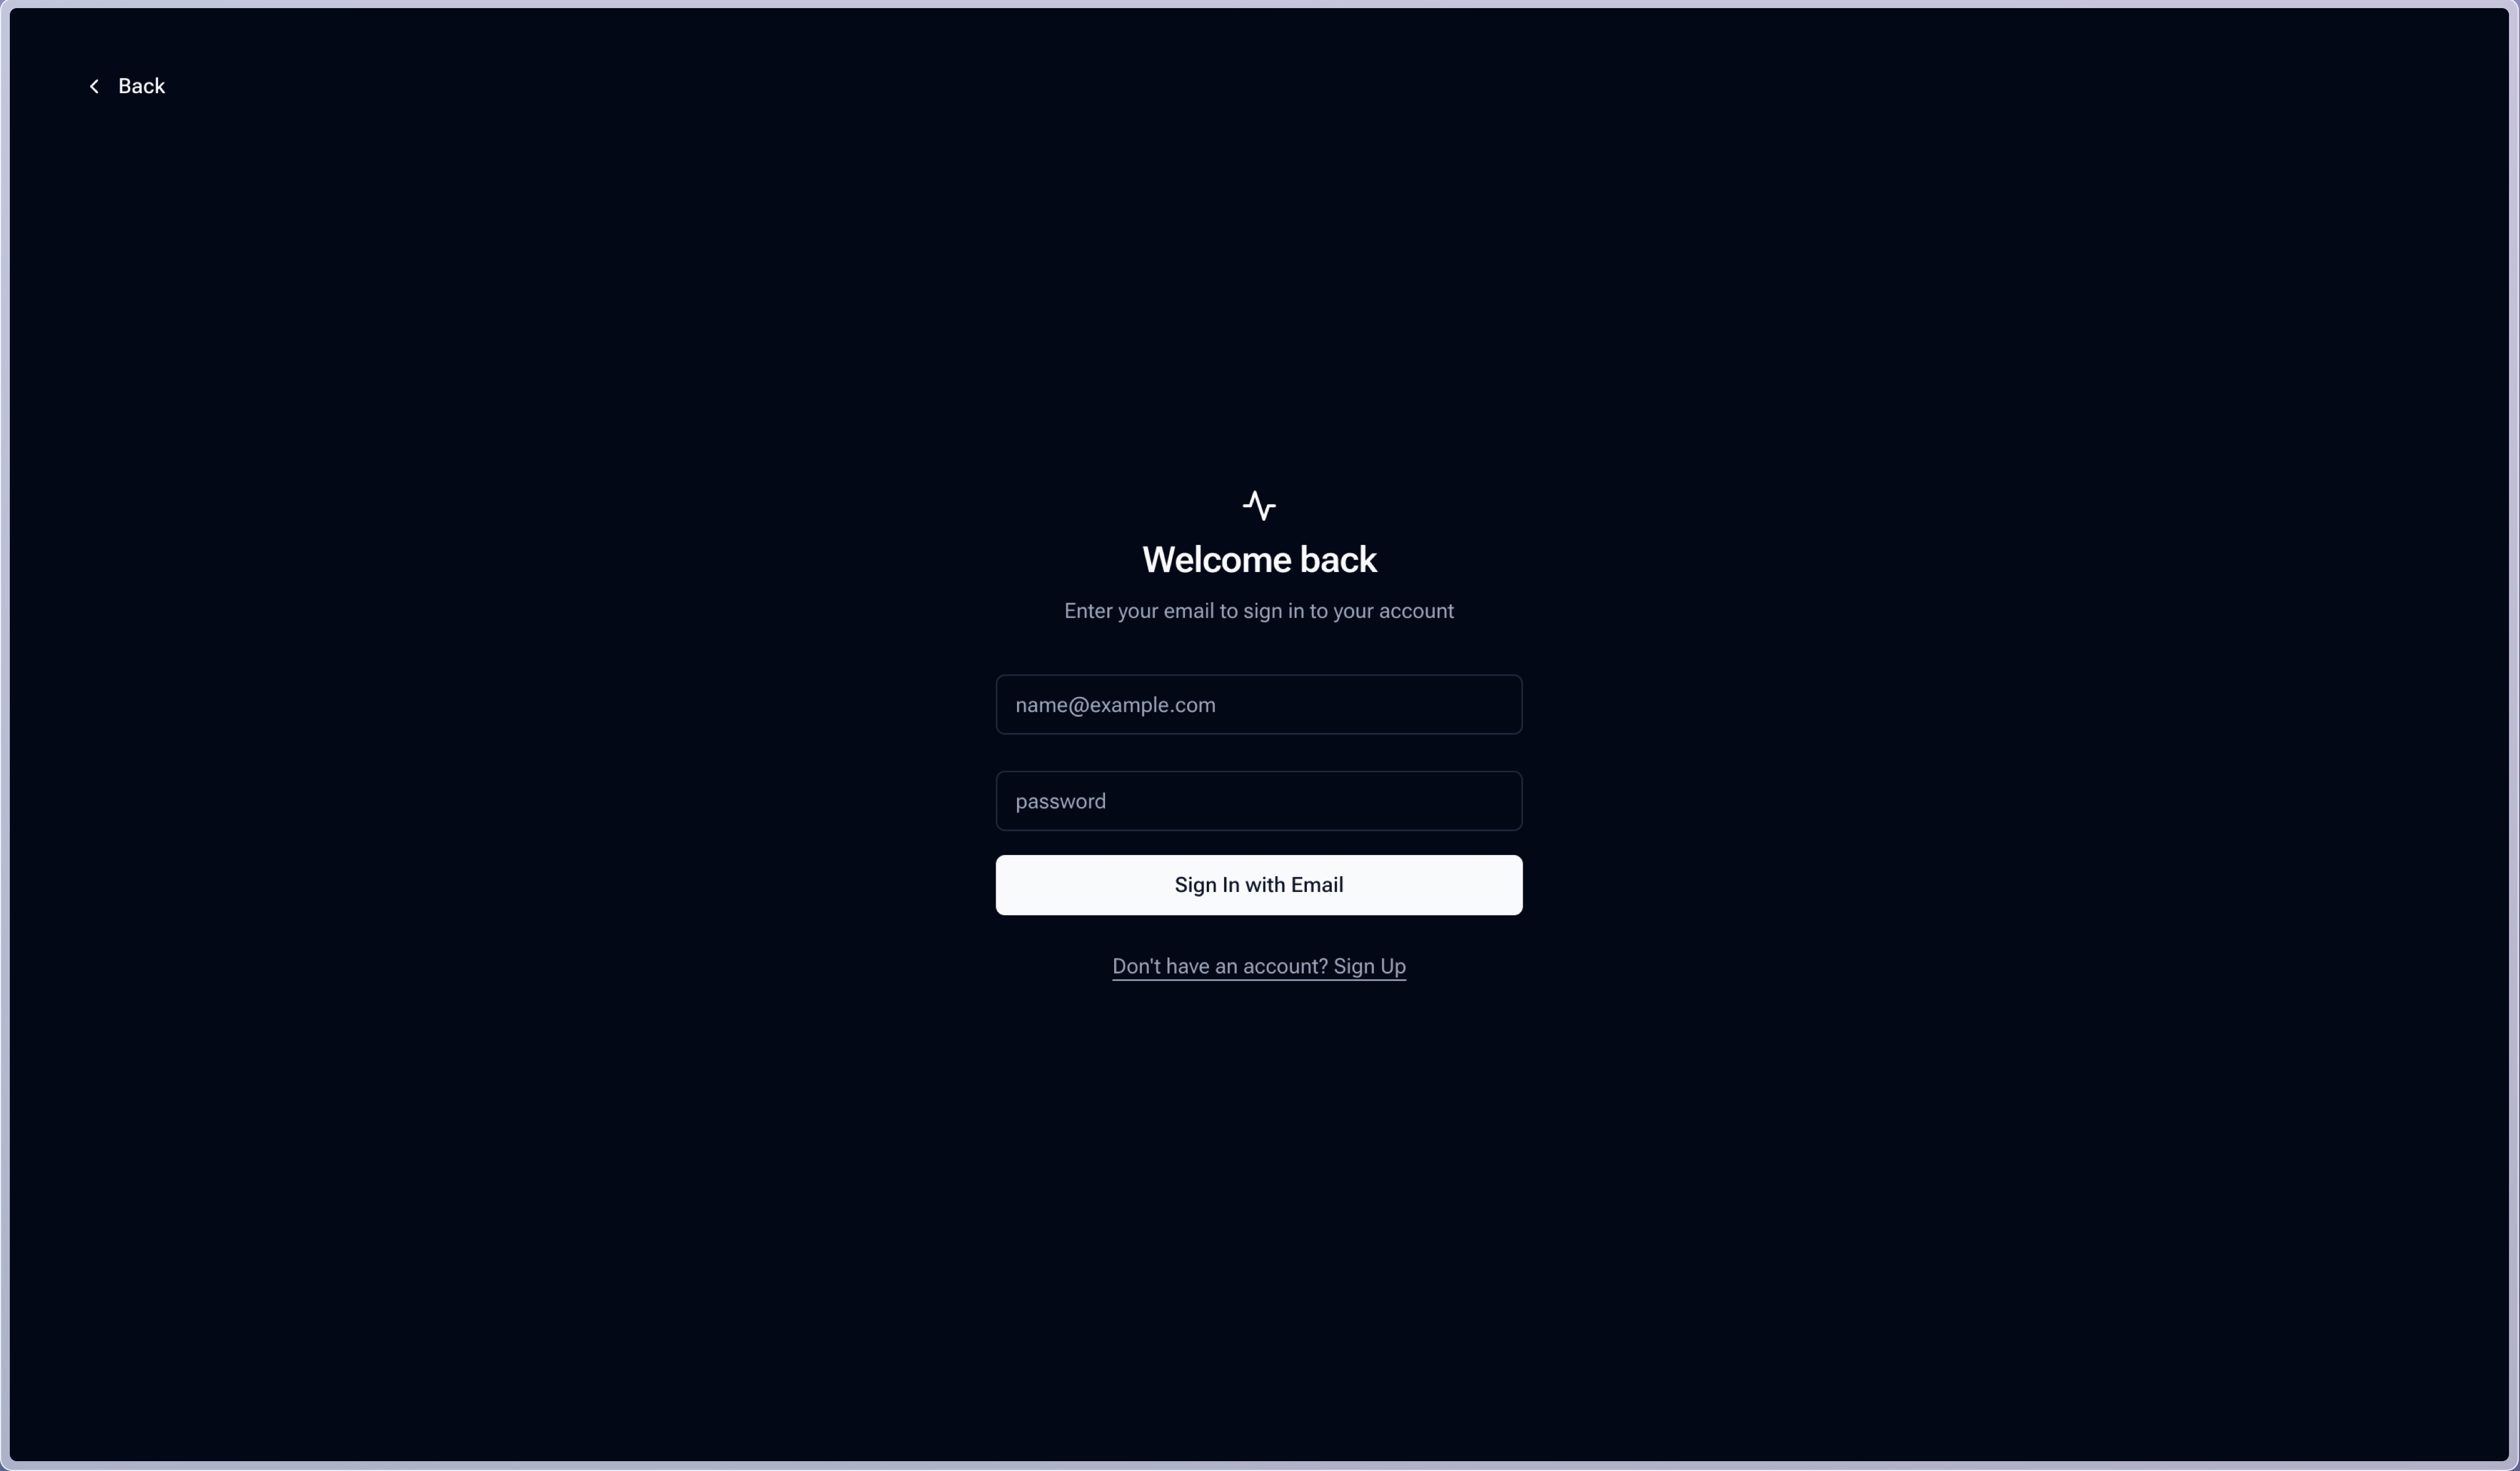
\includegraphics[height=6cm]{figures/fyp_login.jpeg}
  \captionsetup{justification=centering}
  \caption[Webapp Login]{The login screen for the webapp} \label{fig:webapp_login}
\end{figure}
When users first navigate to the website, they are greeted with either the login screen (\autoref{fig:webapp_login}), or the register screen (\autoref{fig:webapp_register}). The login screen is simple, with only two fields, one for the user's email address, and one for their password. The register screen is similarly simple, with fields for the user's name, email address, and password. Users are also required to agree to the consent form and acknowledege they have read the information sheet provided by a PDF link. The consent form and information sheet were written as part of the ethics approval obtained to collect user information. Once the user has registered, they are automatically logged in and redirected to the dashboard screen.
\begin{figure}[htbp]
  \centering
  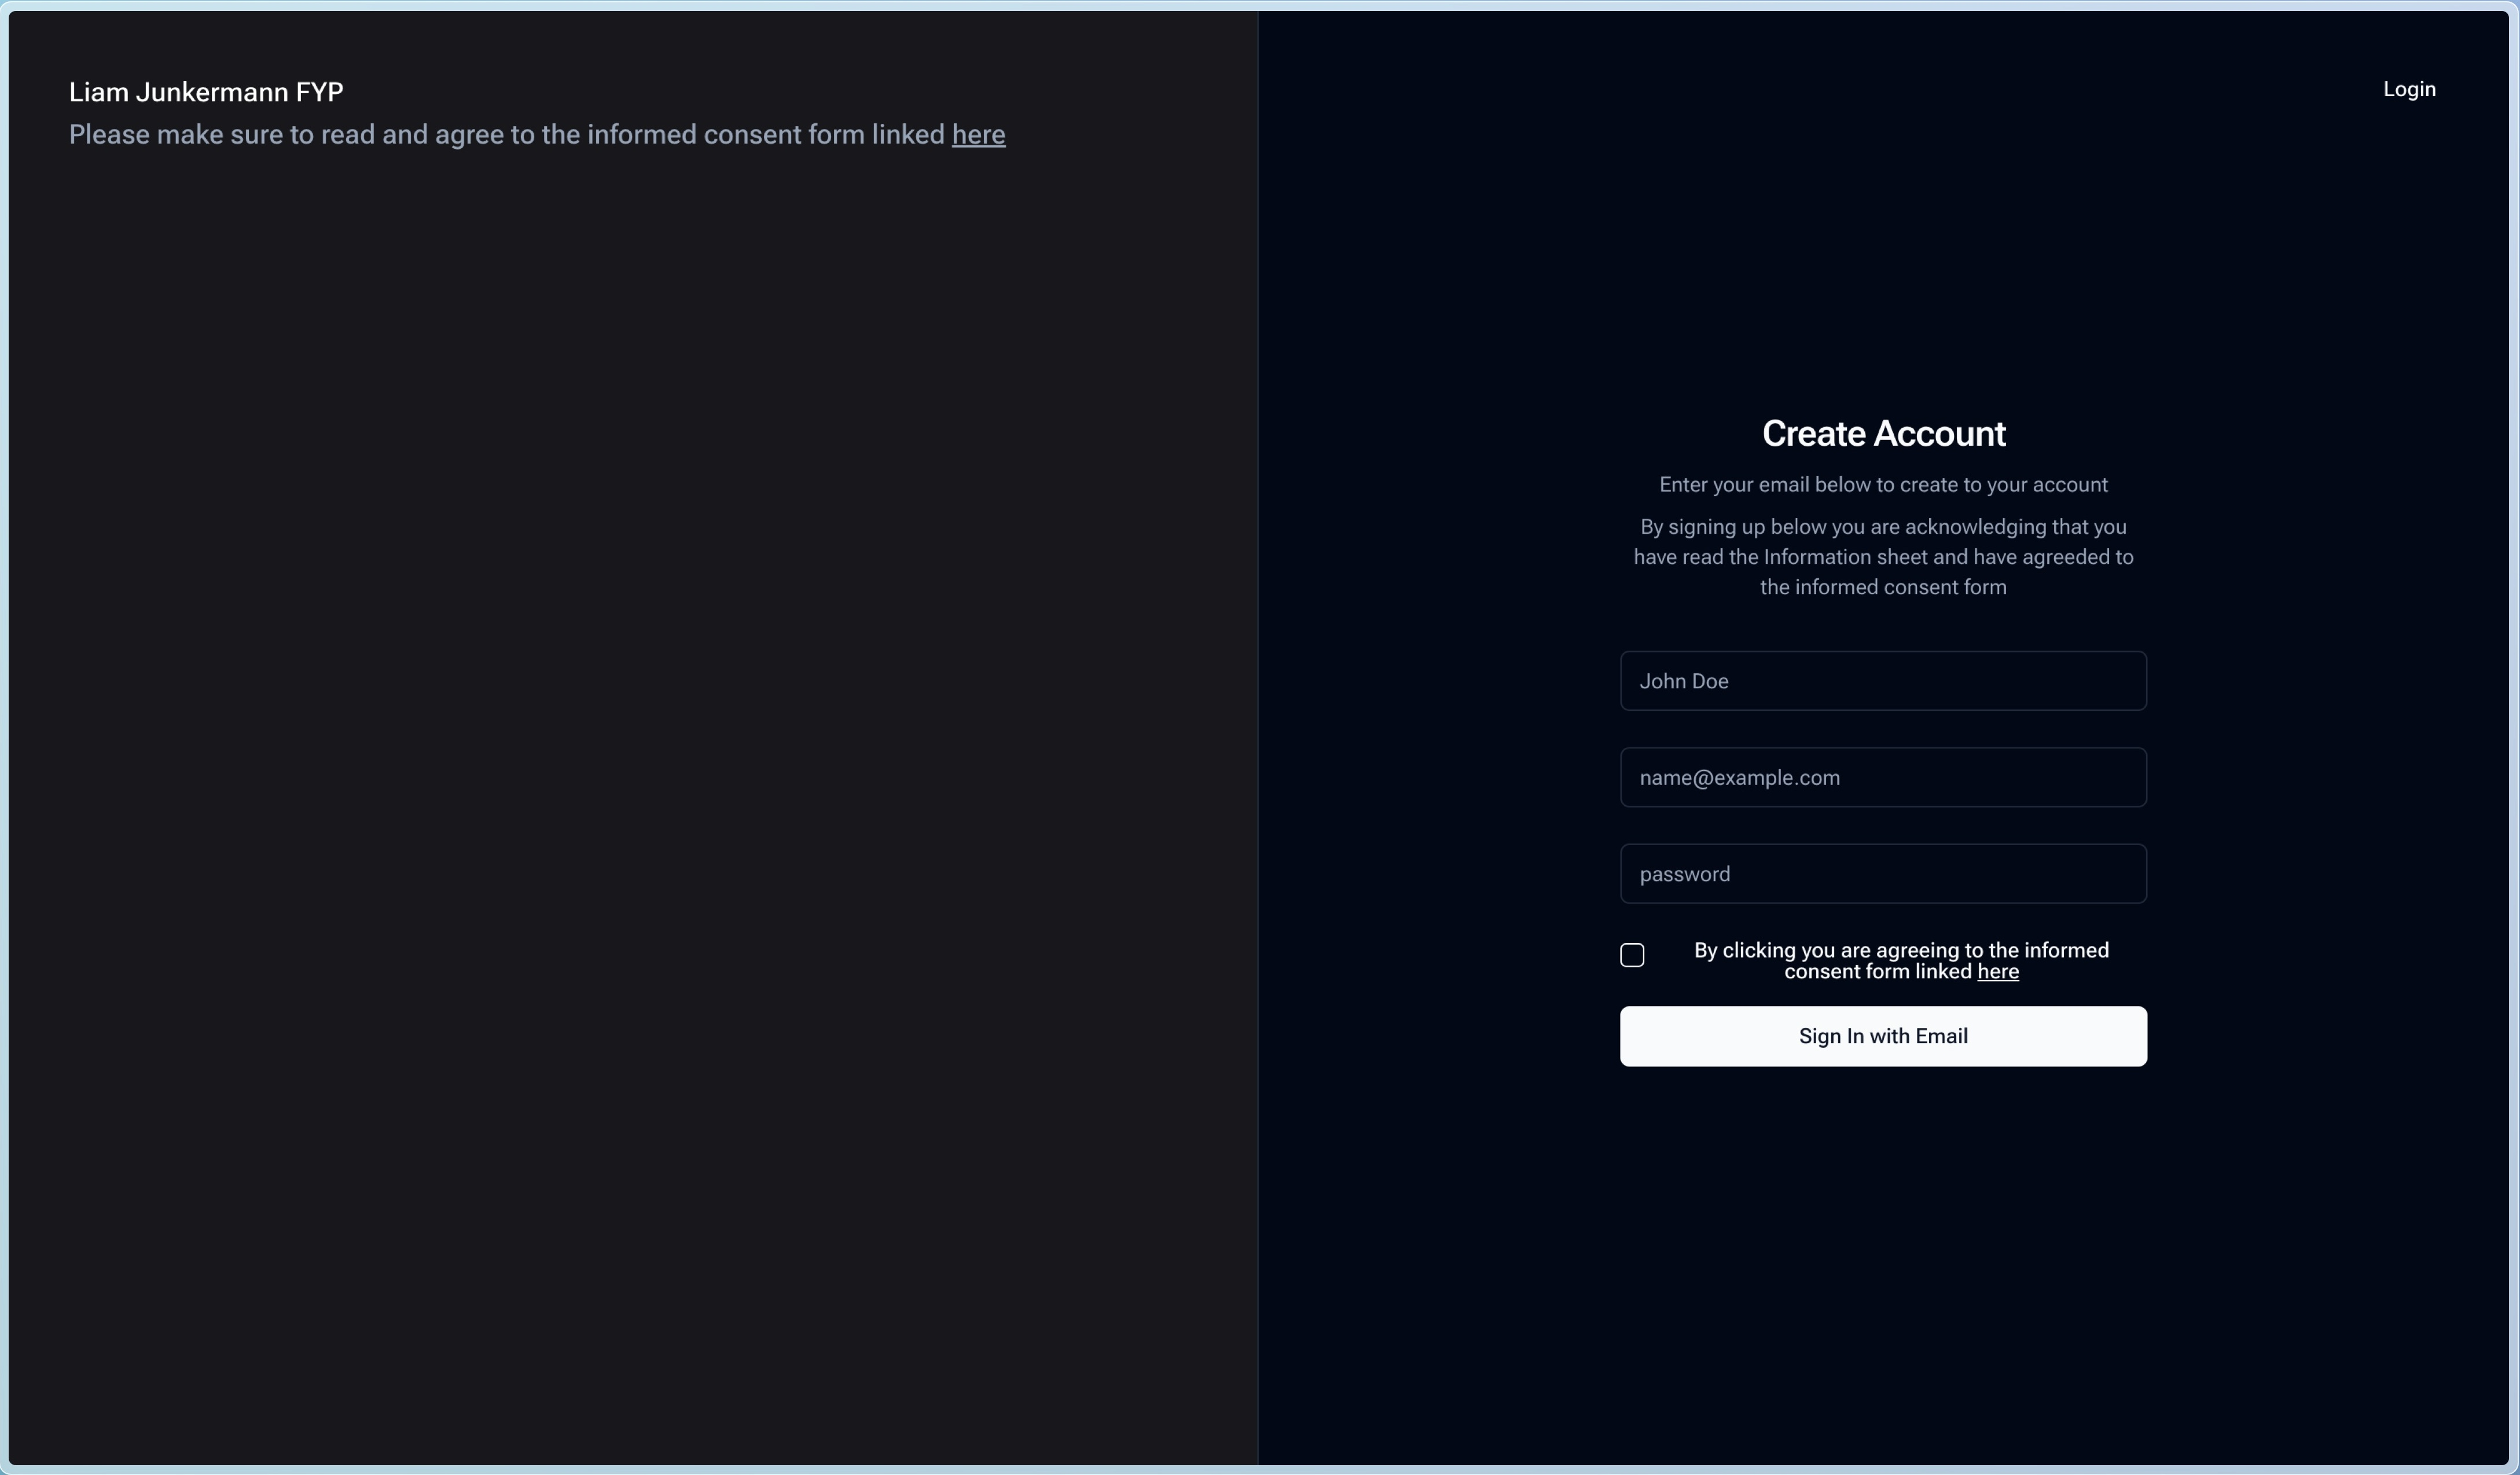
\includegraphics[height=6cm]{figures/fyp_register.jpeg}
  \captionsetup{justification=centering}
  \caption[Webapp Register]{The user registration screen for the webapp} \label{fig:webapp_register}
\end{figure}
\subsubsection{Dashboard}

\begin{figure}[htbp]
  \centering
  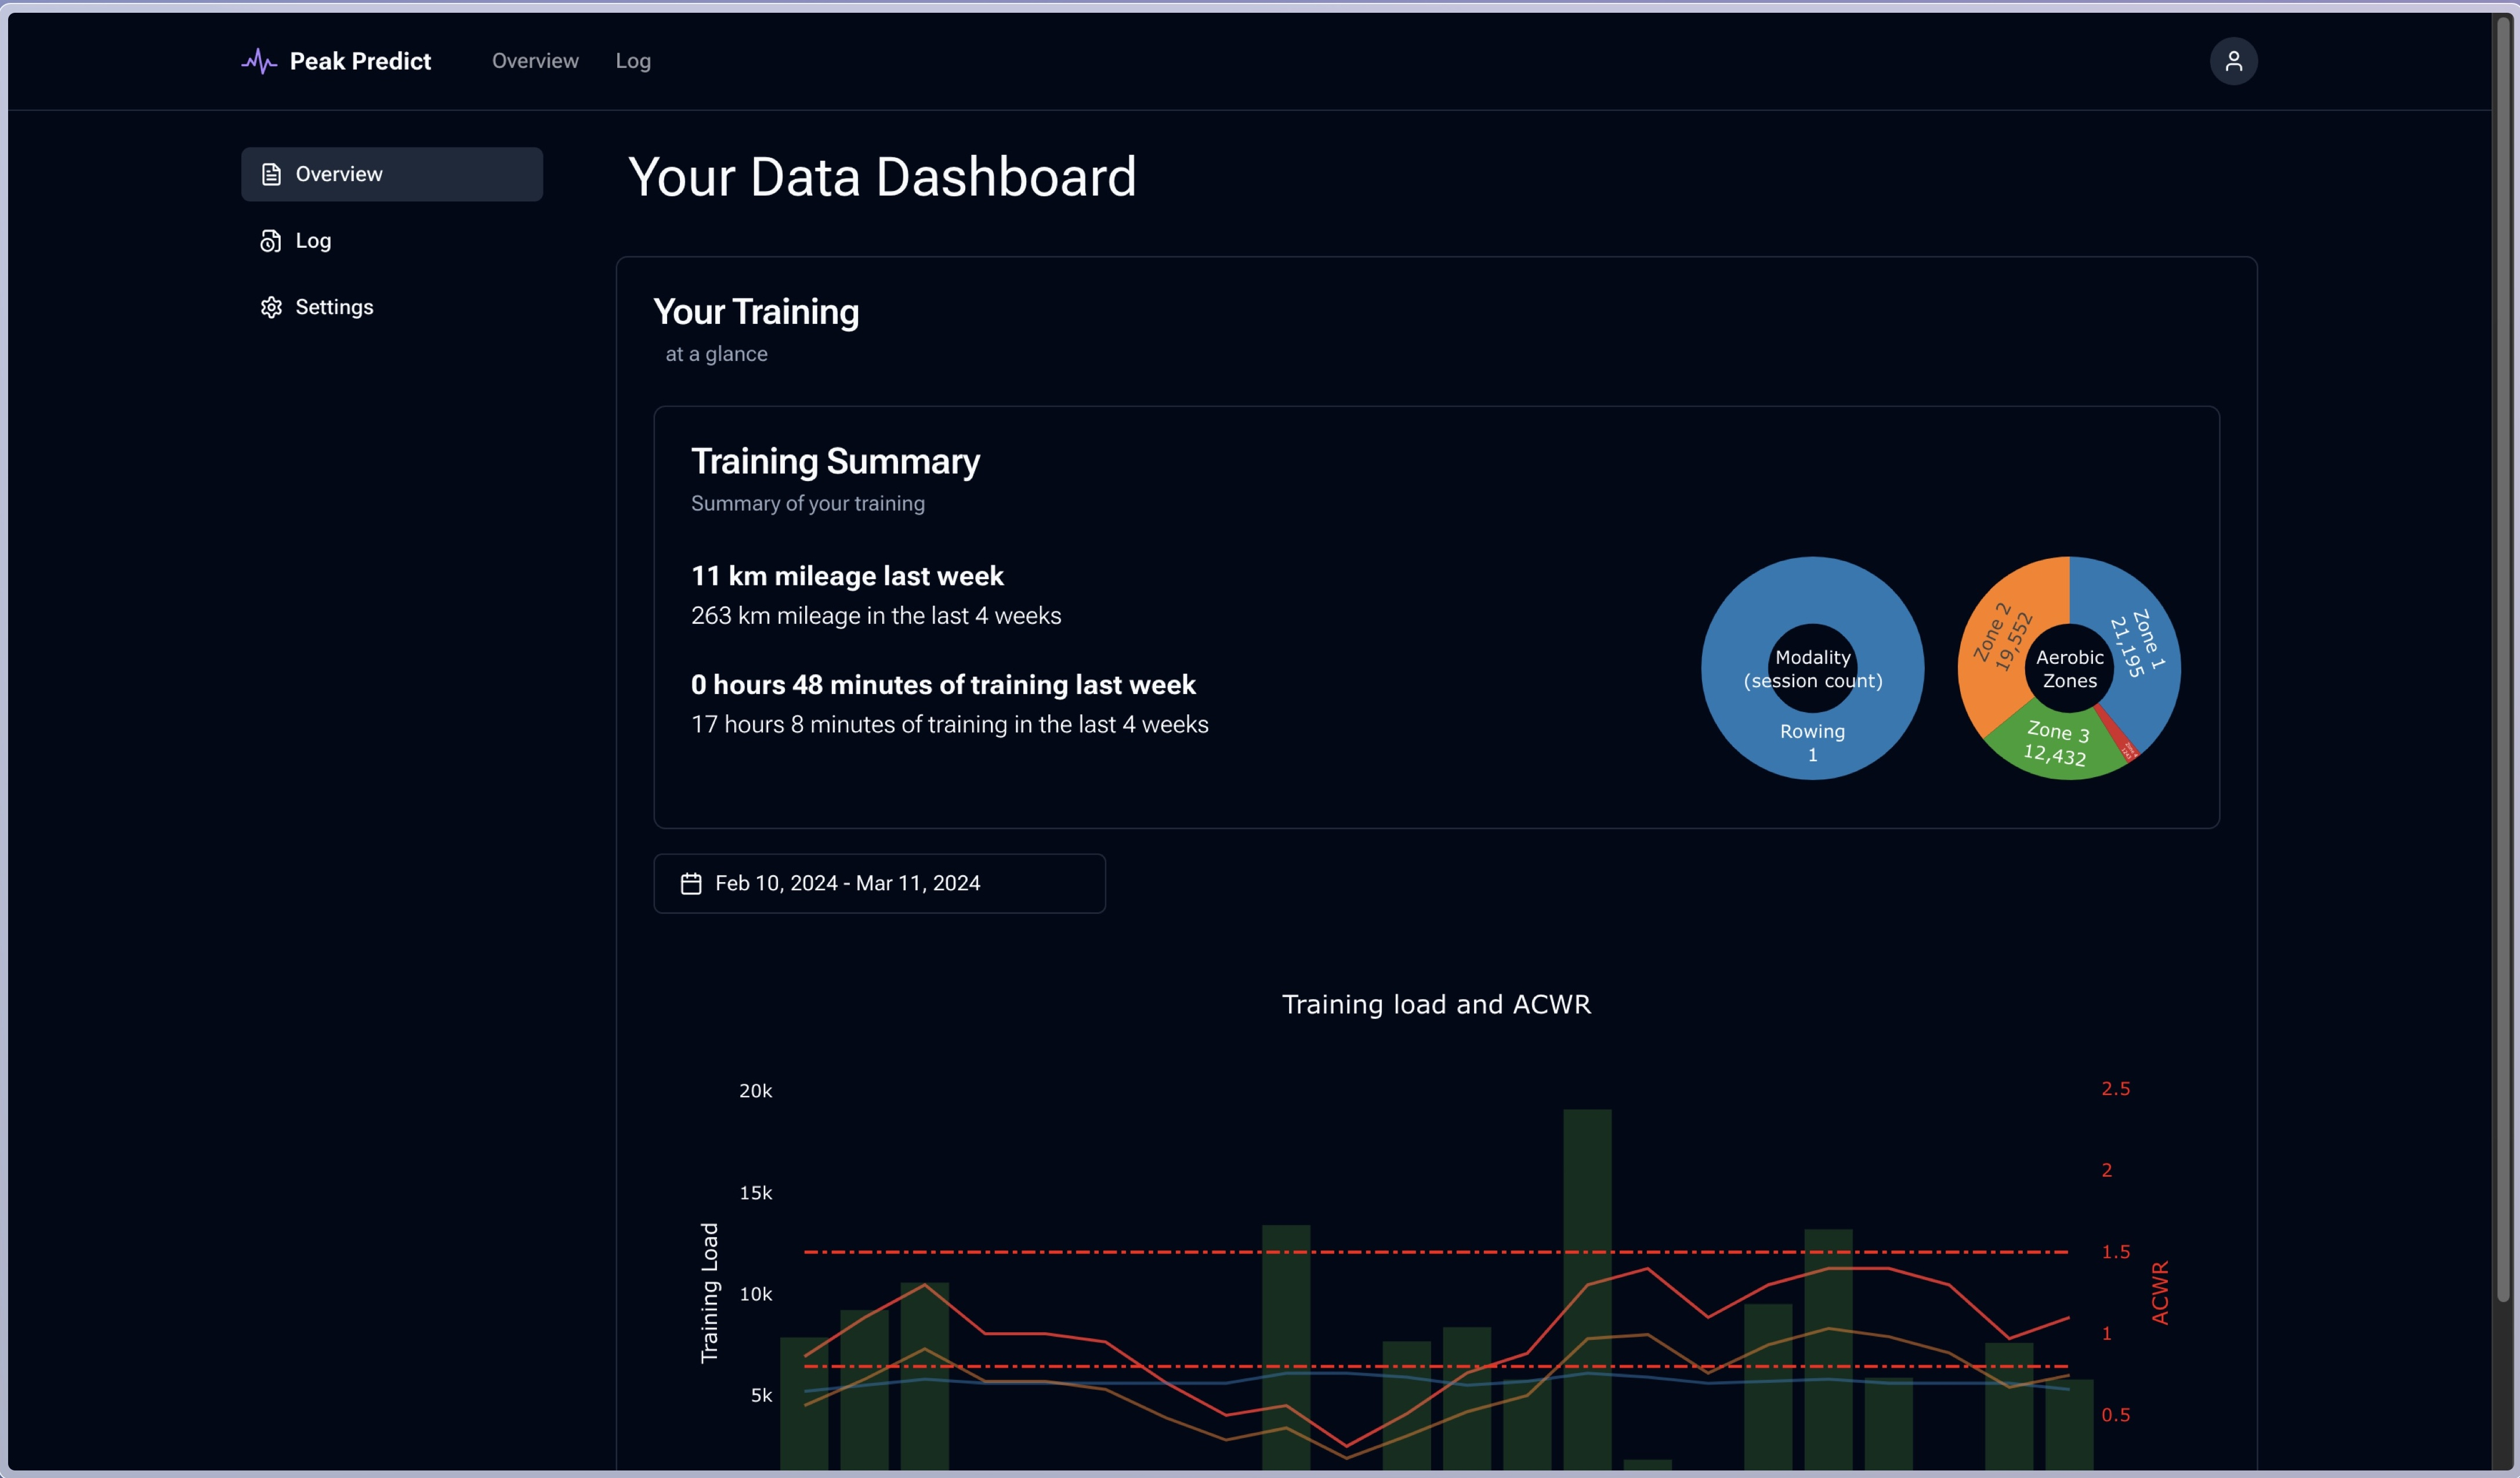
\includegraphics[height=6cm]{figures/fyp_dash_overview.jpeg}
  \captionsetup{justification=centering}
  \caption[Webapp Dashboard]{The dashboard screen for the webapp} \label{fig:webapp_dashboard}
\end{figure}

Once logged in, users are greeted with a dashboard screen (\autoref{fig:webapp_dashboard}). This screen gives a summary of training in the last seven days, as well as some visualisations across a selected time period of the user's choice. At a glance, athletes are able to identify if they are training sustainably, and compare, week-to-week, their mileage and modality break-down. Managing training load is particularly important for rowers as overtraining has even greater knock-on effects in other aspects of a rowers life, like work or college.

\subsubsection{Training Log}

\begin{figure}[htbp]
  \centering
  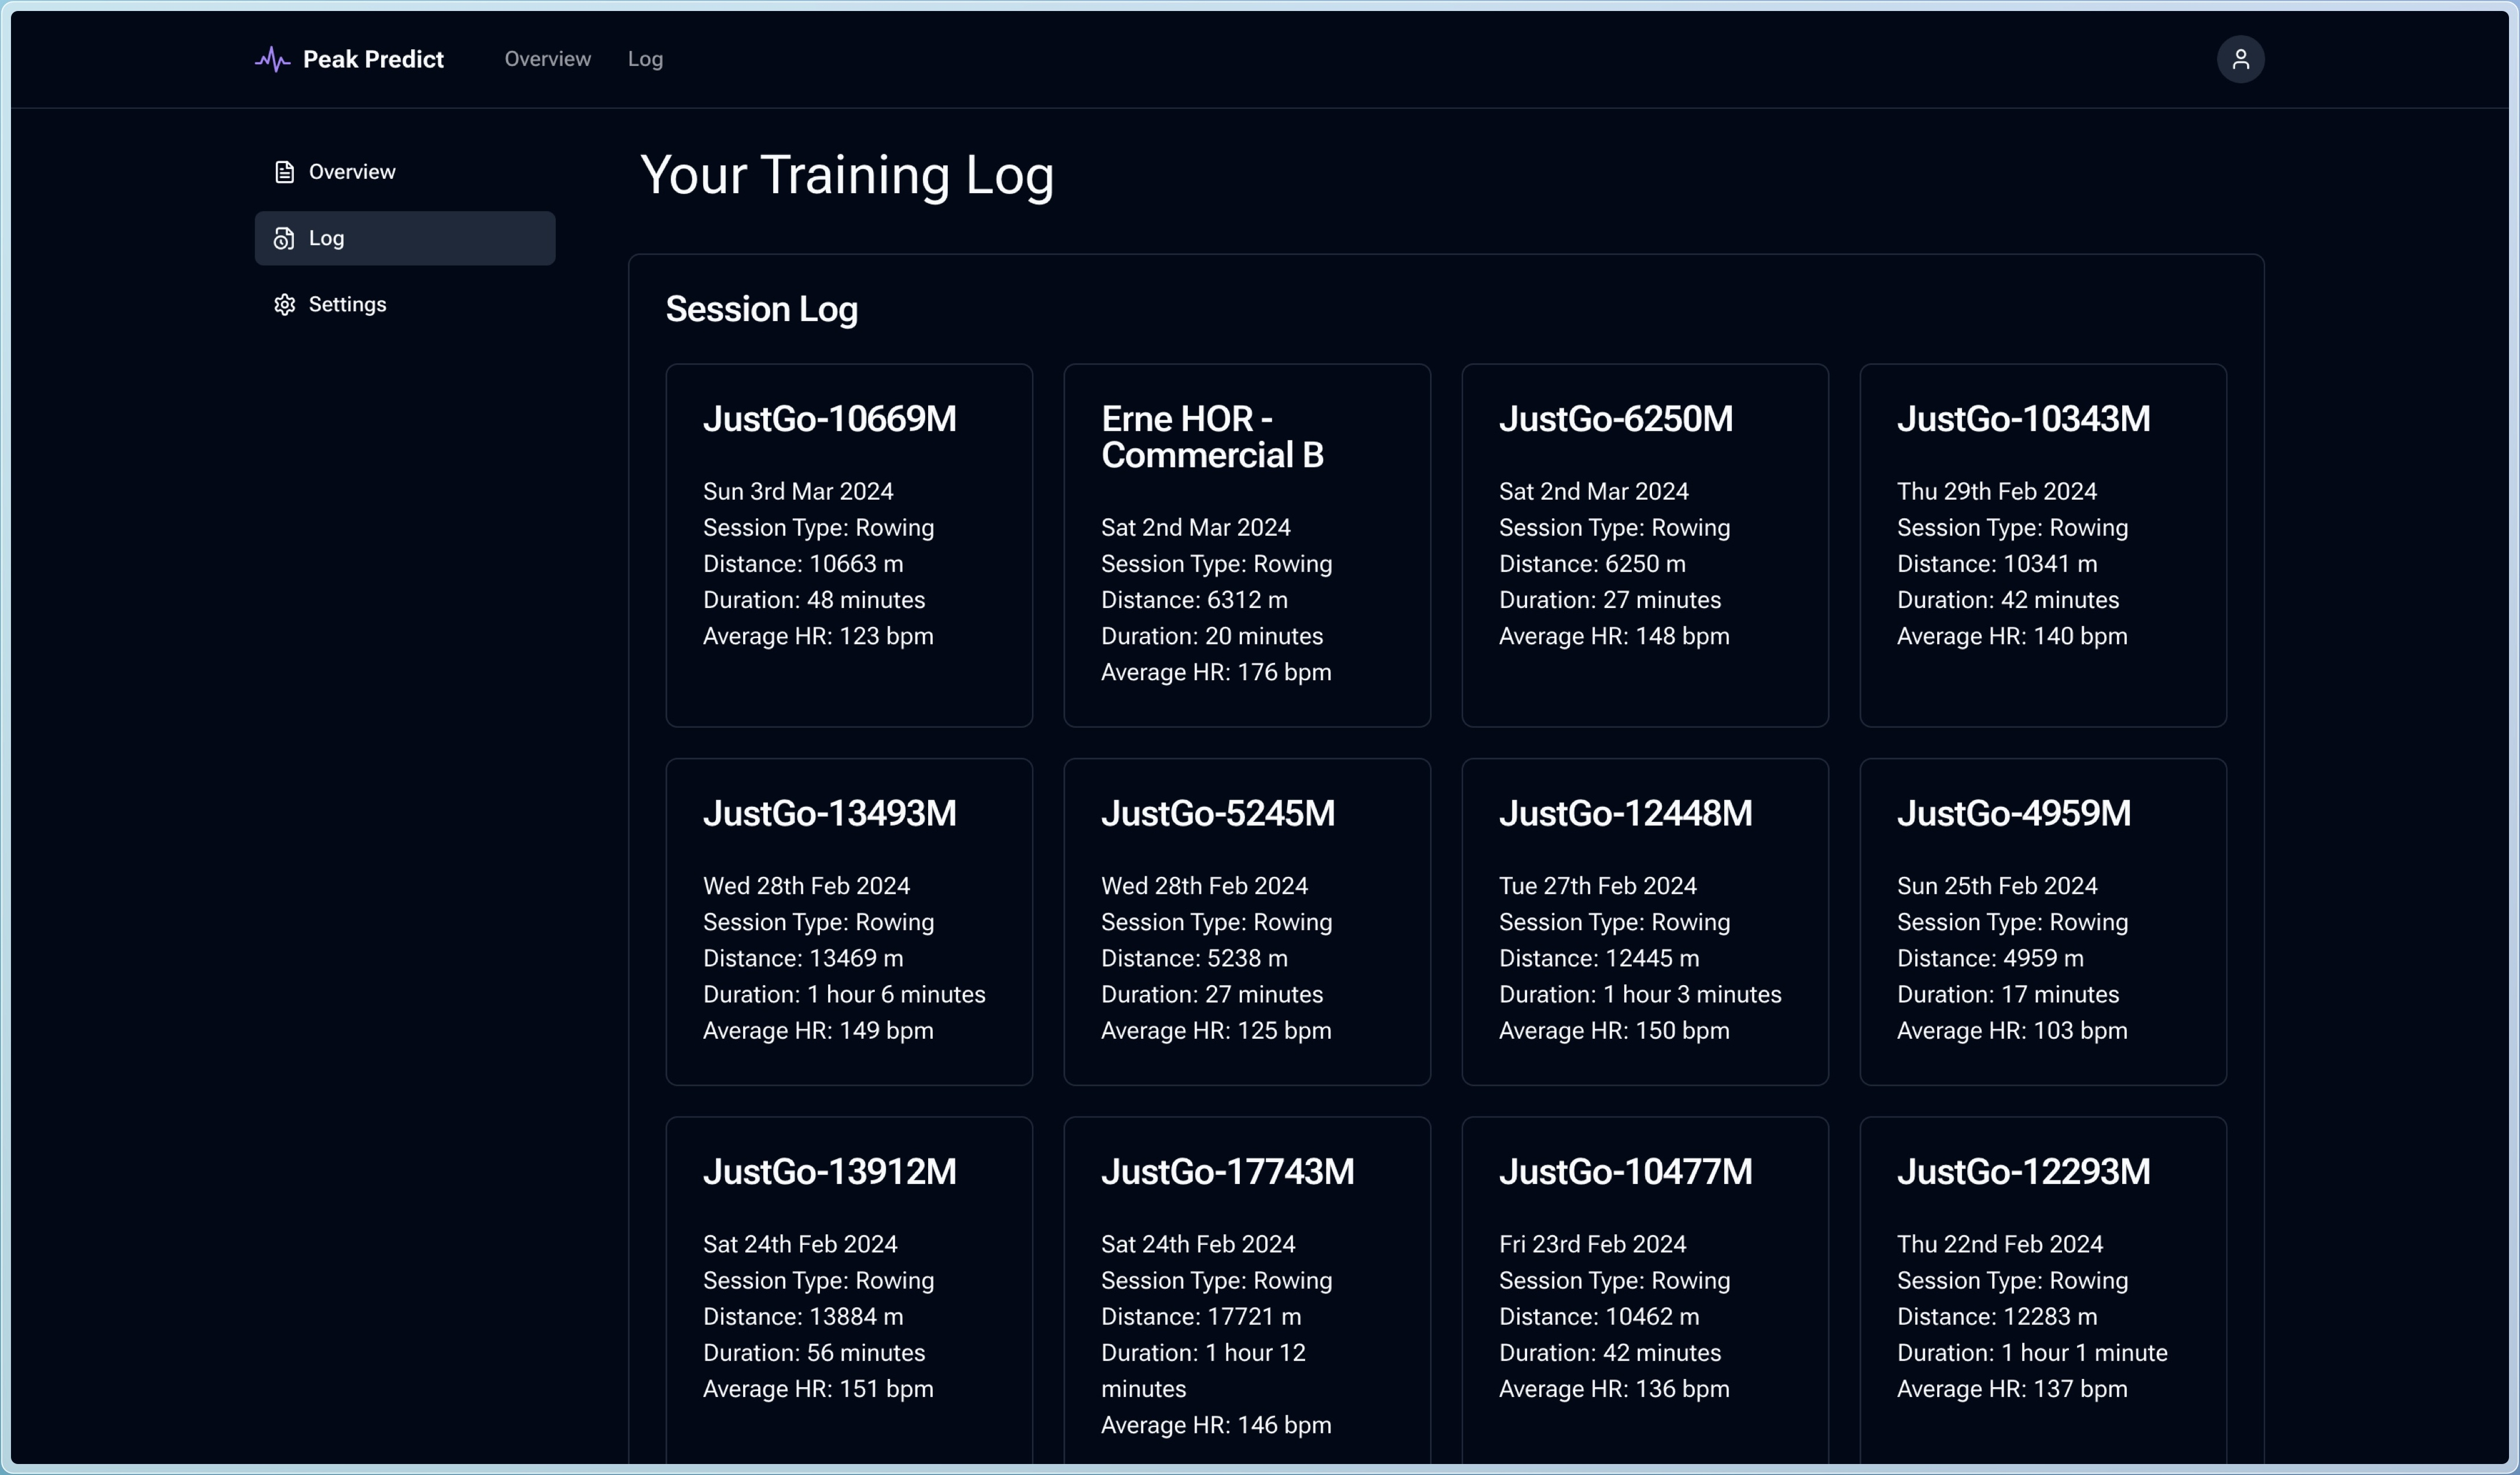
\includegraphics[height=6cm]{figures/fyp_training_log.jpeg}
  \captionsetup{justification=centering}
  \caption[Webapp Training Log]{The training log screen for the webapp} \label{fig:webapp_training_log}
\end{figure}
The training log (\autoref{fig:webapp_training_log}) provides a detailed view of all the sessions a rower has completed. This project did not require athletes to provide additional feedback for sessions, however this page would host a form to allow athletes to add sessions and session feedback in a more developed version of the webapp, this will be discussed more in the Discussion, \autoref{chap:discussion}. The user can also click on a session to view more detailed information about that session, including heart rate data, GPS data, and any other data collected during the session. 

\subsubsection{Connections Manager}

\begin{figure}[htbp]
  \centering
  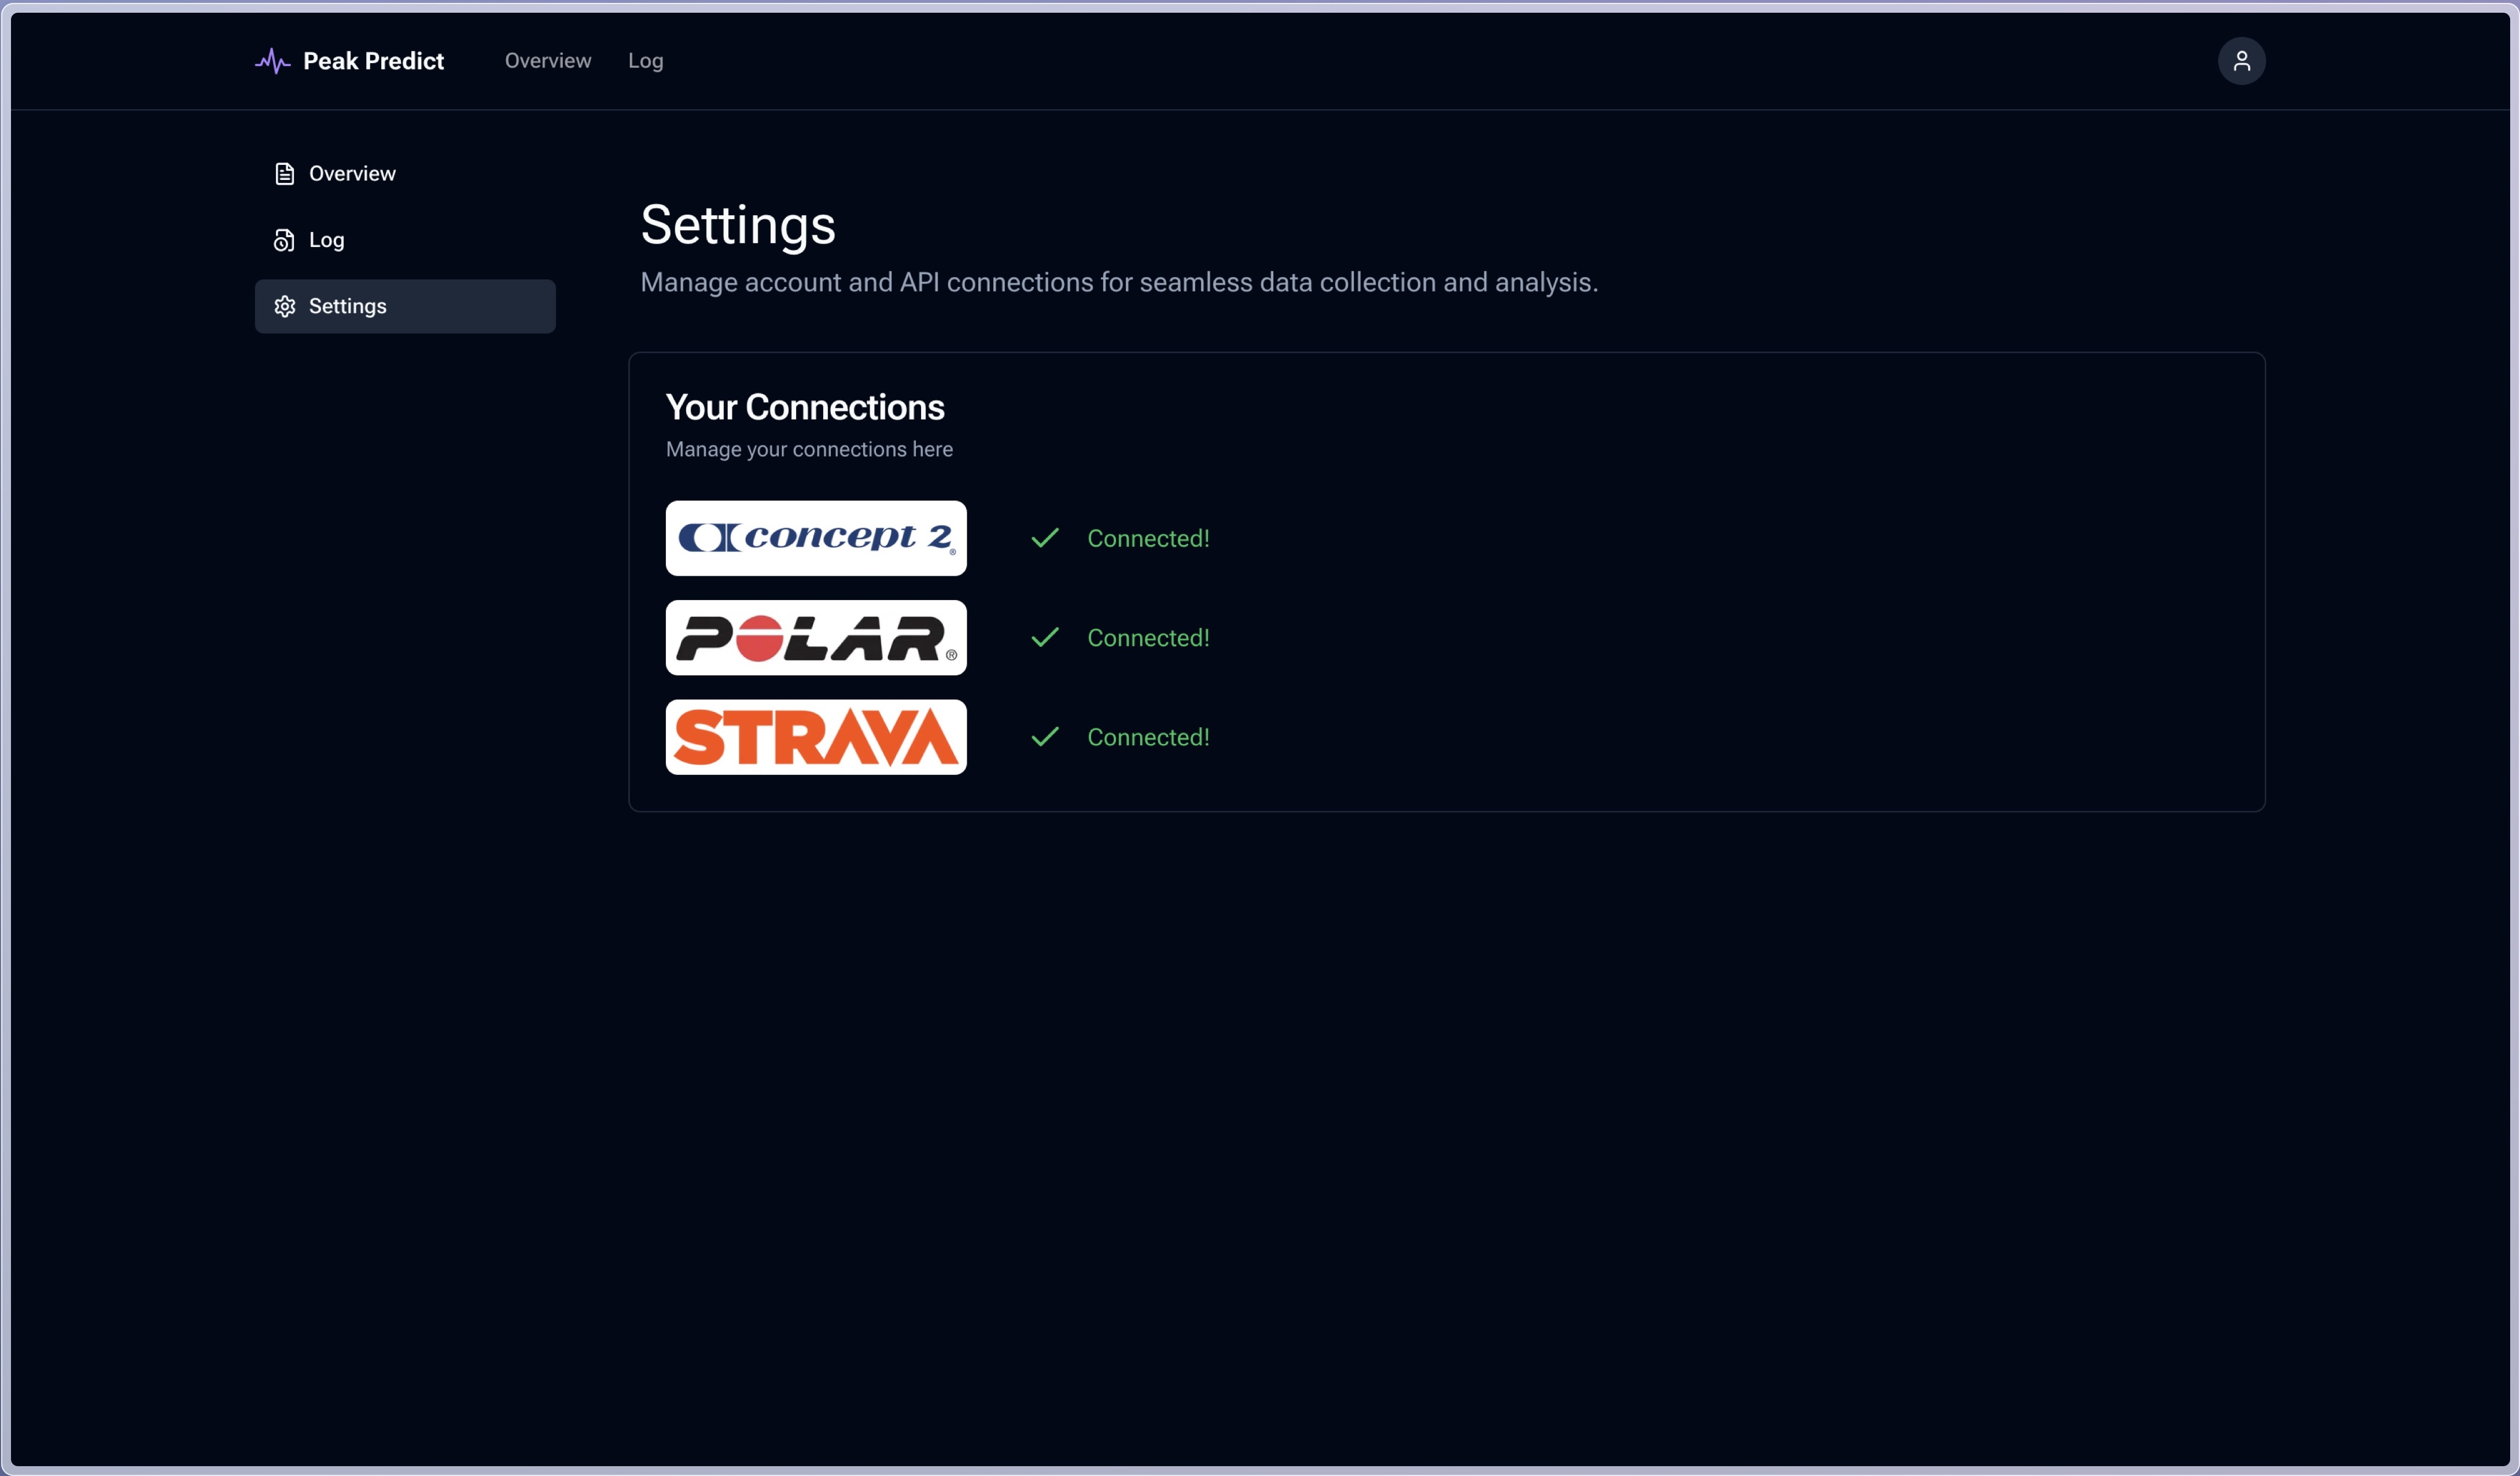
\includegraphics[height=6cm]{figures/fyp_connections_page.jpeg}
  \captionsetup{justification=centering}
  \caption[Webapp Connections Manager]{\label{fig:webapp_connection_mgr}The connections manager screen for the webapp} 
\end{figure}
The final screen in the app is the settings page (\autoref{fig:webapp_connection_mgr}), which is home to the connections manager. Here users can see which data providers they have connected. This page is where the most user interaction happened throughout the project. Given the goal of minimal user intervention and maintanence, when logging in for the first time they were directed to this page to connect their rowing data providers, and using the OAuth protocol, shared the necessary keys with the project to allow data to flow automatically in the backend.  

\subsection{The Backend}
The backend services were crucial to developing a system that required minimal user and maintainer intervention. The backend was developed using serverless functions, which are small, single-purpose functions that are run in response to events. These functions were used to collect data from the user's data providers, analyse the data, and generate feedback for the user. The backend was developed using the Serverless framework, which is a framework for building serverless applications. The backend was hosted on AWS, and used a combination of AWS Lambda, AWS API Gateway, AWS DynamoDB, and AWS S3 to provide the serverless functions, and store the data. The backend functions were primarily built using Node.js and Typesript. This section will only discuss the data collection and management functions. Analysis functions will be discussed in the Data Analysis and Visualisation chapter, \autoref{chap:data-analysis-viz}.

There are 4 major functions, which were separated into serverless functions to manage and handle data. These functions are the Provider Connection, Provider Webhooks, Data Ingestor, and Data Processor. Each of these functions is responsible for a different part of the data collection and management process.

The general webapp backend was mostly handled by AWS Amplify. This service made it possible for the researcher to focus on providing valuable features to users, rather than spending extra time developing boilerplate authentication and database interactions. The Amplify service also provided a GraphQL API, which was used to interact with the DynamoDB database, and provided a simple way to interact with the database from the frontend in a secure way.

\subsubsection{Provider Connection}
When connecting to a service using the OAuth protocol, the user is redirected to the service's login page, where they log in and authorise the project to access their data. Once the user has authorised the project, the service redirects the user back to the project's website, and provides an access token that can be used to access the user's data. This access token is then stored in the database, and is used to access the user's data in the future. This function is responsible for handling the OAuth flow, and storing the access token in the database. The provider connection function handles the various data formats which different providers use, and connects access and refresh tokens to the users for use later on in the pipeline when activities are generated. This particular function was built as part of the Next.js server, leveraging the server-side rendering capabilities of the framework to handle authentication of users using cookies making the linking of tokens with users easier.

\subsubsection{Provider Webhooks}
Typically when a user completes a workout, the data provider can query a webhook (if it has been set up), with a payload containing basic information about the workout, and in some cases, the details to retrieve the full session. For each of the supported data providers, Polar, Concept2, and Strava, webhooks were setup and registered with the providers. Webhooks were then handled through the Next.js server, retrieving any additional data needed. The full session data was then shared to the Data Ingestor function for processing and storage in the database. Different providers had different requirements for the webhook payload, and the data was stored in different formats, so the webhook function was responsible for handling these differences and normalising the data before sending it to the Data Ingestor function, while also limiting the unnecessary sharing of client secrets and keys across multiple services.

\subsubsection{Data Ingestor}
The data ingestor handled the actual storage of the data in the database. The data ingestor first validated any data provided. This was done by validating the provider user id and comparing a key which was shared with the Next.js server. Then it stored the raw session data, provided by the webhook handler in the Next.js server, in AWS S3, this meant that any issues with data processing could be rectified after the fact with the raw data available. Finally, the ingestor triggered the Data Processor function. This extra level of data processing before storing the data ensured that data ingested to the data pipeline was legitimate and provided through the proper channel. This function was a standalone serverless function, built using Node.js and Typescript, and deployed to AWS Lambda using the Serverless framework.

\subsubsection{Data Processor}
Given the variety of data and session types provided, a standard exercise model was needed to make analysis and machine learning easier. The data processor function was responsible for taking the raw session data, and converting it into a standard format. The standard format included a sessions duration, distance, average heart rate (if applicable), time of completion, session type, and session modality. These features would be used to complete analysis and produce the weekly training summaries shown in the frontend. This was also a standalone serverless function, built using Node.js and Typescript, and deployed to AWS Lambda using the Serverless framework.

\section{Data Management}
Given the expected volume of data collected, the design of how to store and manage this data was important to ensuring analysis could happen quickly, and AWS costs remained low. Almost all the data stored was already provided in a structured JSON format, originally these data responses were saved and stored in AWS S3. This allowed the researcher time to understand what data was being collected, and what was important. From this, the Standard Exercise Model was derived. This model was then used to create a DynamoDB table to store the data in a structured format. The data was stored in a table with the schema described in \autoref{tab:std_exercise_model}.
\begin{table}[h]
  \centering
  \resizebox{\textwidth}{!}{%
  \begin{tabular}{lll}
  \textbf{Column Name} & \textbf{Column Data Type} & \textbf{Description} \\
  \texttt{owner} & \texttt{string} & The users uid \\
  \texttt{exercise\_id} & \texttt{string} & An autogenerated id. The tables primary key \\
  \texttt{data\_source} & \texttt{\{source:~string, path:~string\}{[}{]}} & The raw data source(s) and linked data in S3 \\
  \texttt{datetime} & \texttt{number} & The unix timestamp for the session \\
  \texttt{type} & \texttt{"endurance" | "interval" | "strength" | "other" | "unknown"} & The session type, an enumerated list \\
  \texttt{modality} & \texttt{"row" | "erg" | "other"} & The session modality, an enumerated list \\
  \texttt{duration} & \texttt{number} & The duration, in seconds, of the session \\
  \texttt{distance} & \texttt{number} & The distance, in meters, of the session \\
  \texttt{avg\_hr} & \texttt{number} & The average HR, in bpm, of the session
  \end{tabular}%
  }
  \caption[Standard Exercise Model Schema]{\label{tab:std_exercise_model}The schema for the "Standard Exercise Model"}
\end{table}

This schema made it particularly easy to perform analysis on each athletes training, distilling the key metrics into a small data size. DynamoDB also allows for robust querying of large datasets, allowing this solution to scale well with lots of data. The data was stored in a single table, with the exercise id as the partition key, and the users unique id as the sort key. This allowed for easy querying of the data, and made it easy to retrieve data for a specific user, or for a specific session. With connections to the raw data included in this data format, more detailed analysis can still be completed automatically, without unnecessary S3 reads to find the session amongst a larger, less dynamic data set. Future work could continue to grow this standard model, adding more features which may be commonly used for analysis, such as time in zones, calculated training impulse, or more. However, for the purposes of providing data for the frontend and the initial analysis, this model was sufficient.

